\section{Low-informative logit model MCMC convergence} \label{app:logit_convergence}
The following section reports the plots and indices used to asses the convergence of our MCMC used to esitame the simple logit model shown in Section \ref{sec:logit}. In \

\begin{figure}[h]
    \centering
    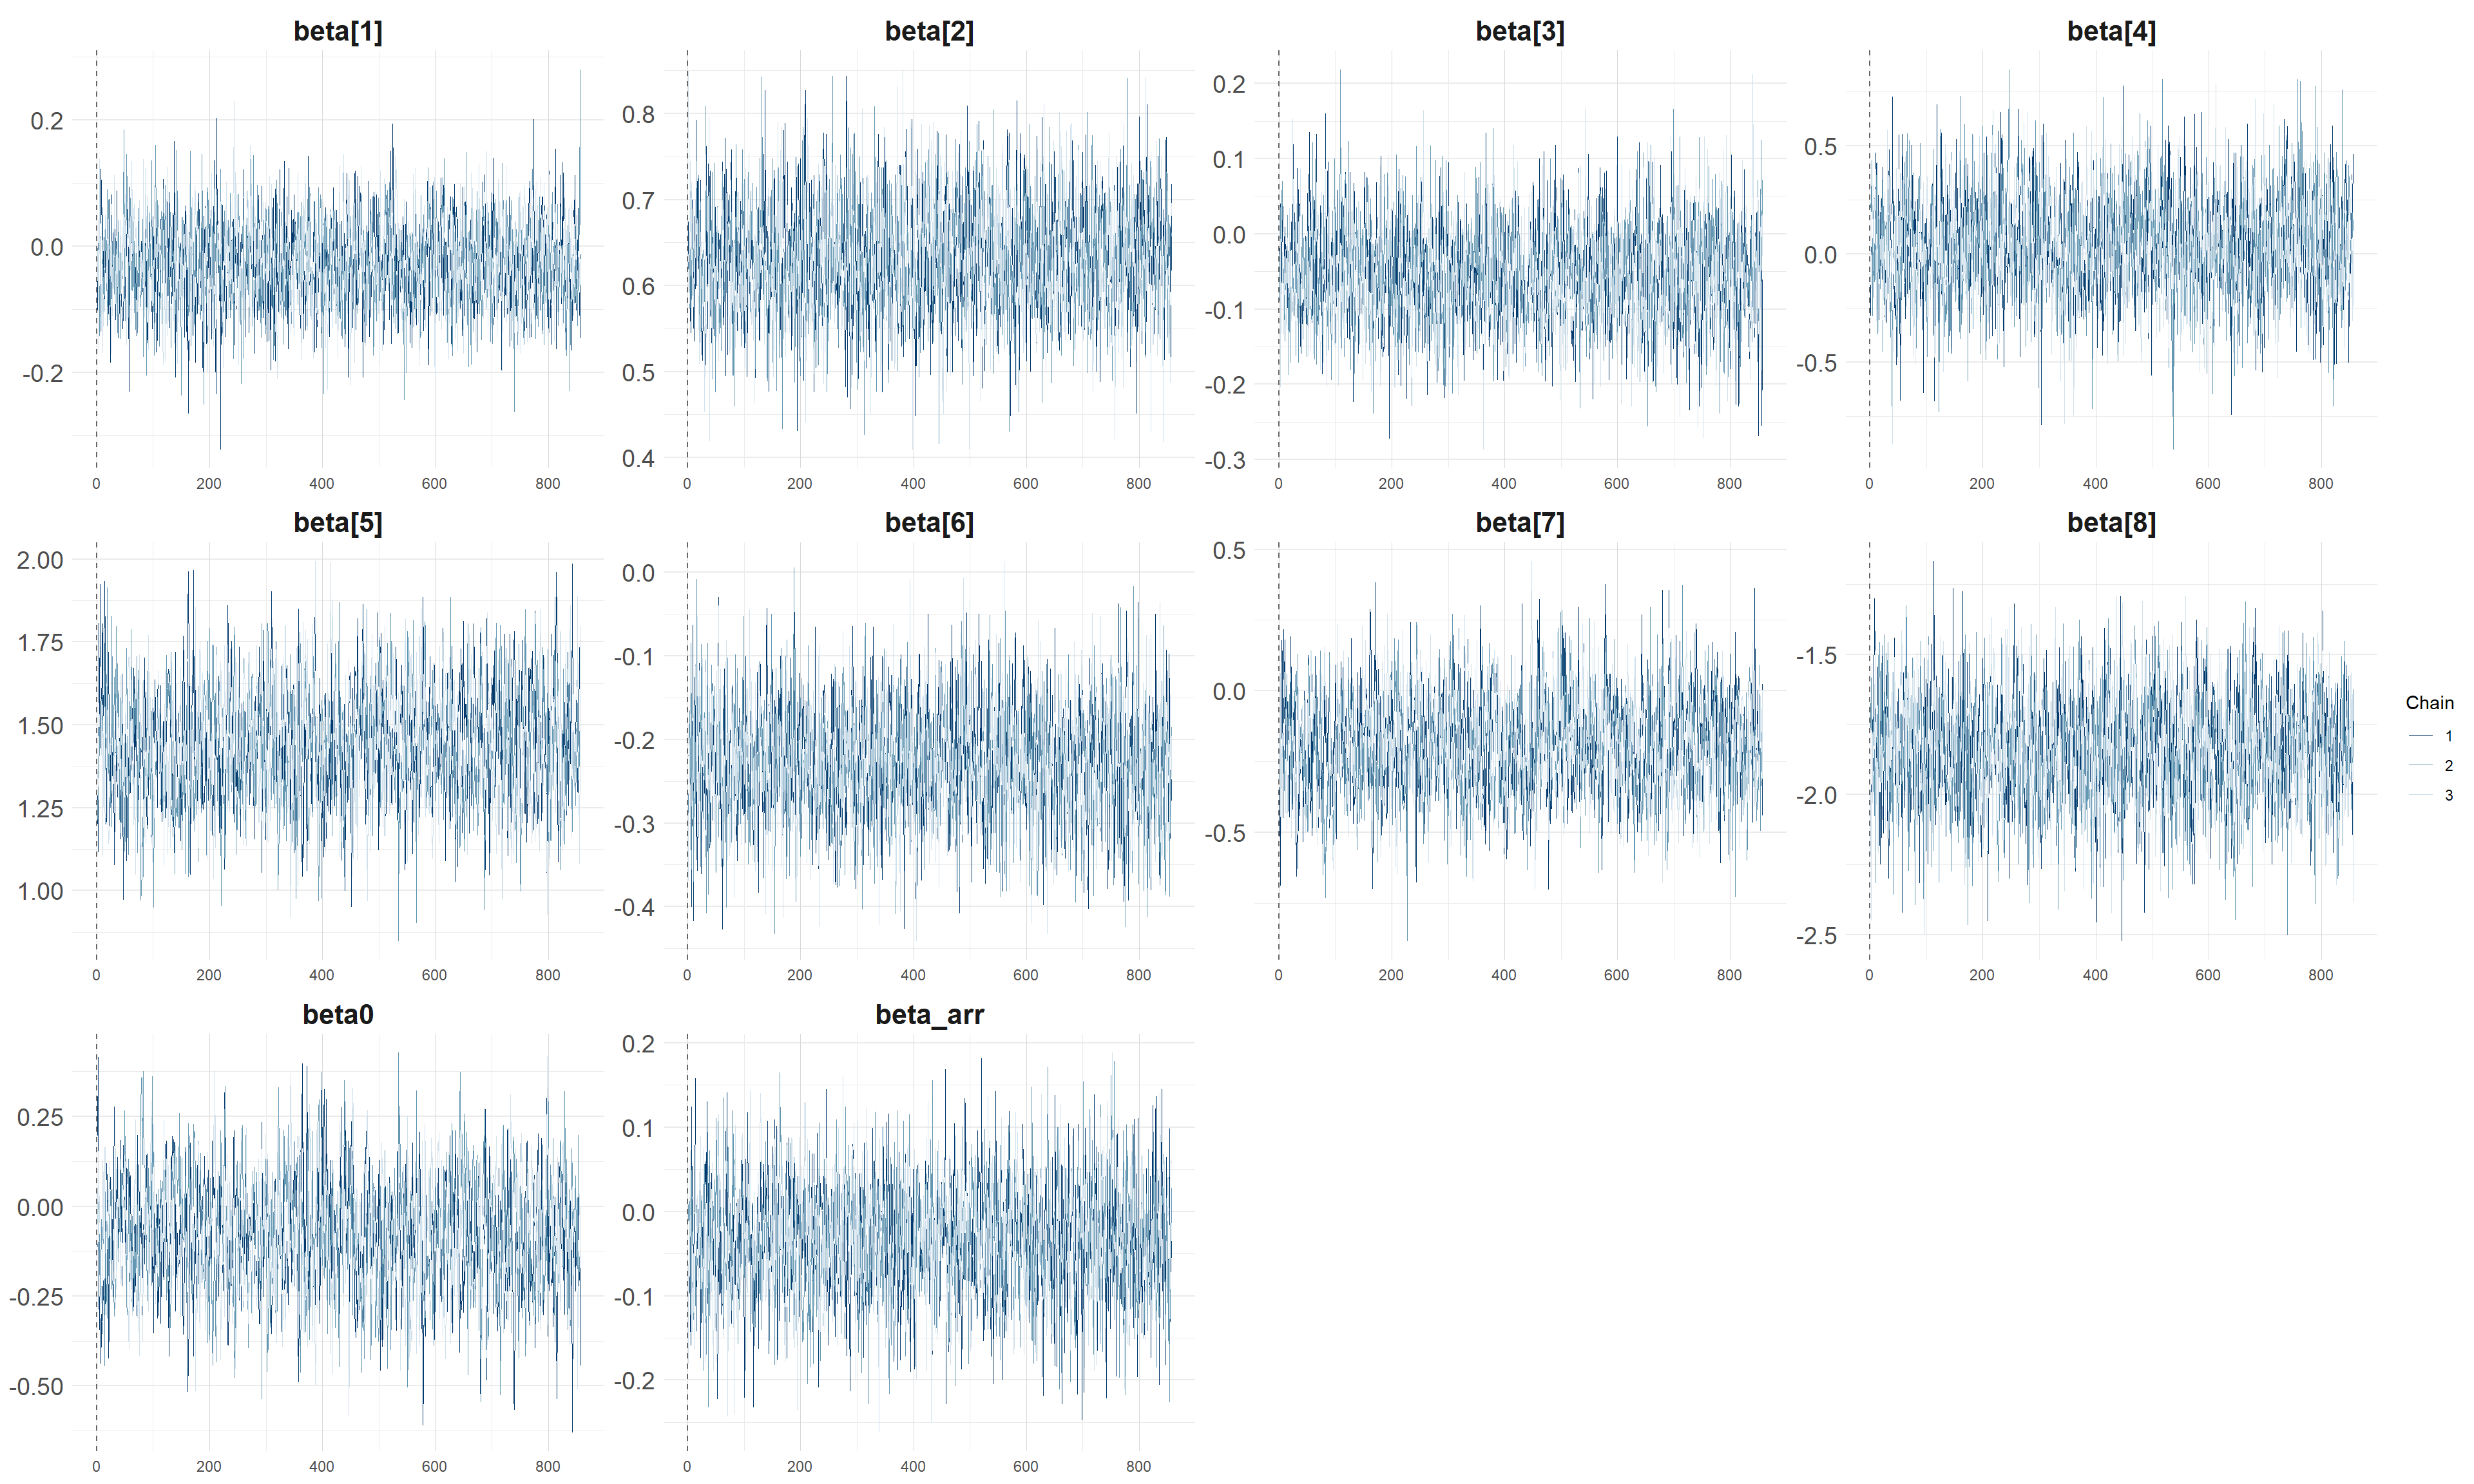
\includegraphics[width=0.9\linewidth]{img/logit_model/trace.png}
    \caption{MCMC traceplot of the baseline logit model.}
    \label{fig:logit_trace}
\end{figure}

\begin{figure}[h]
    \centering
    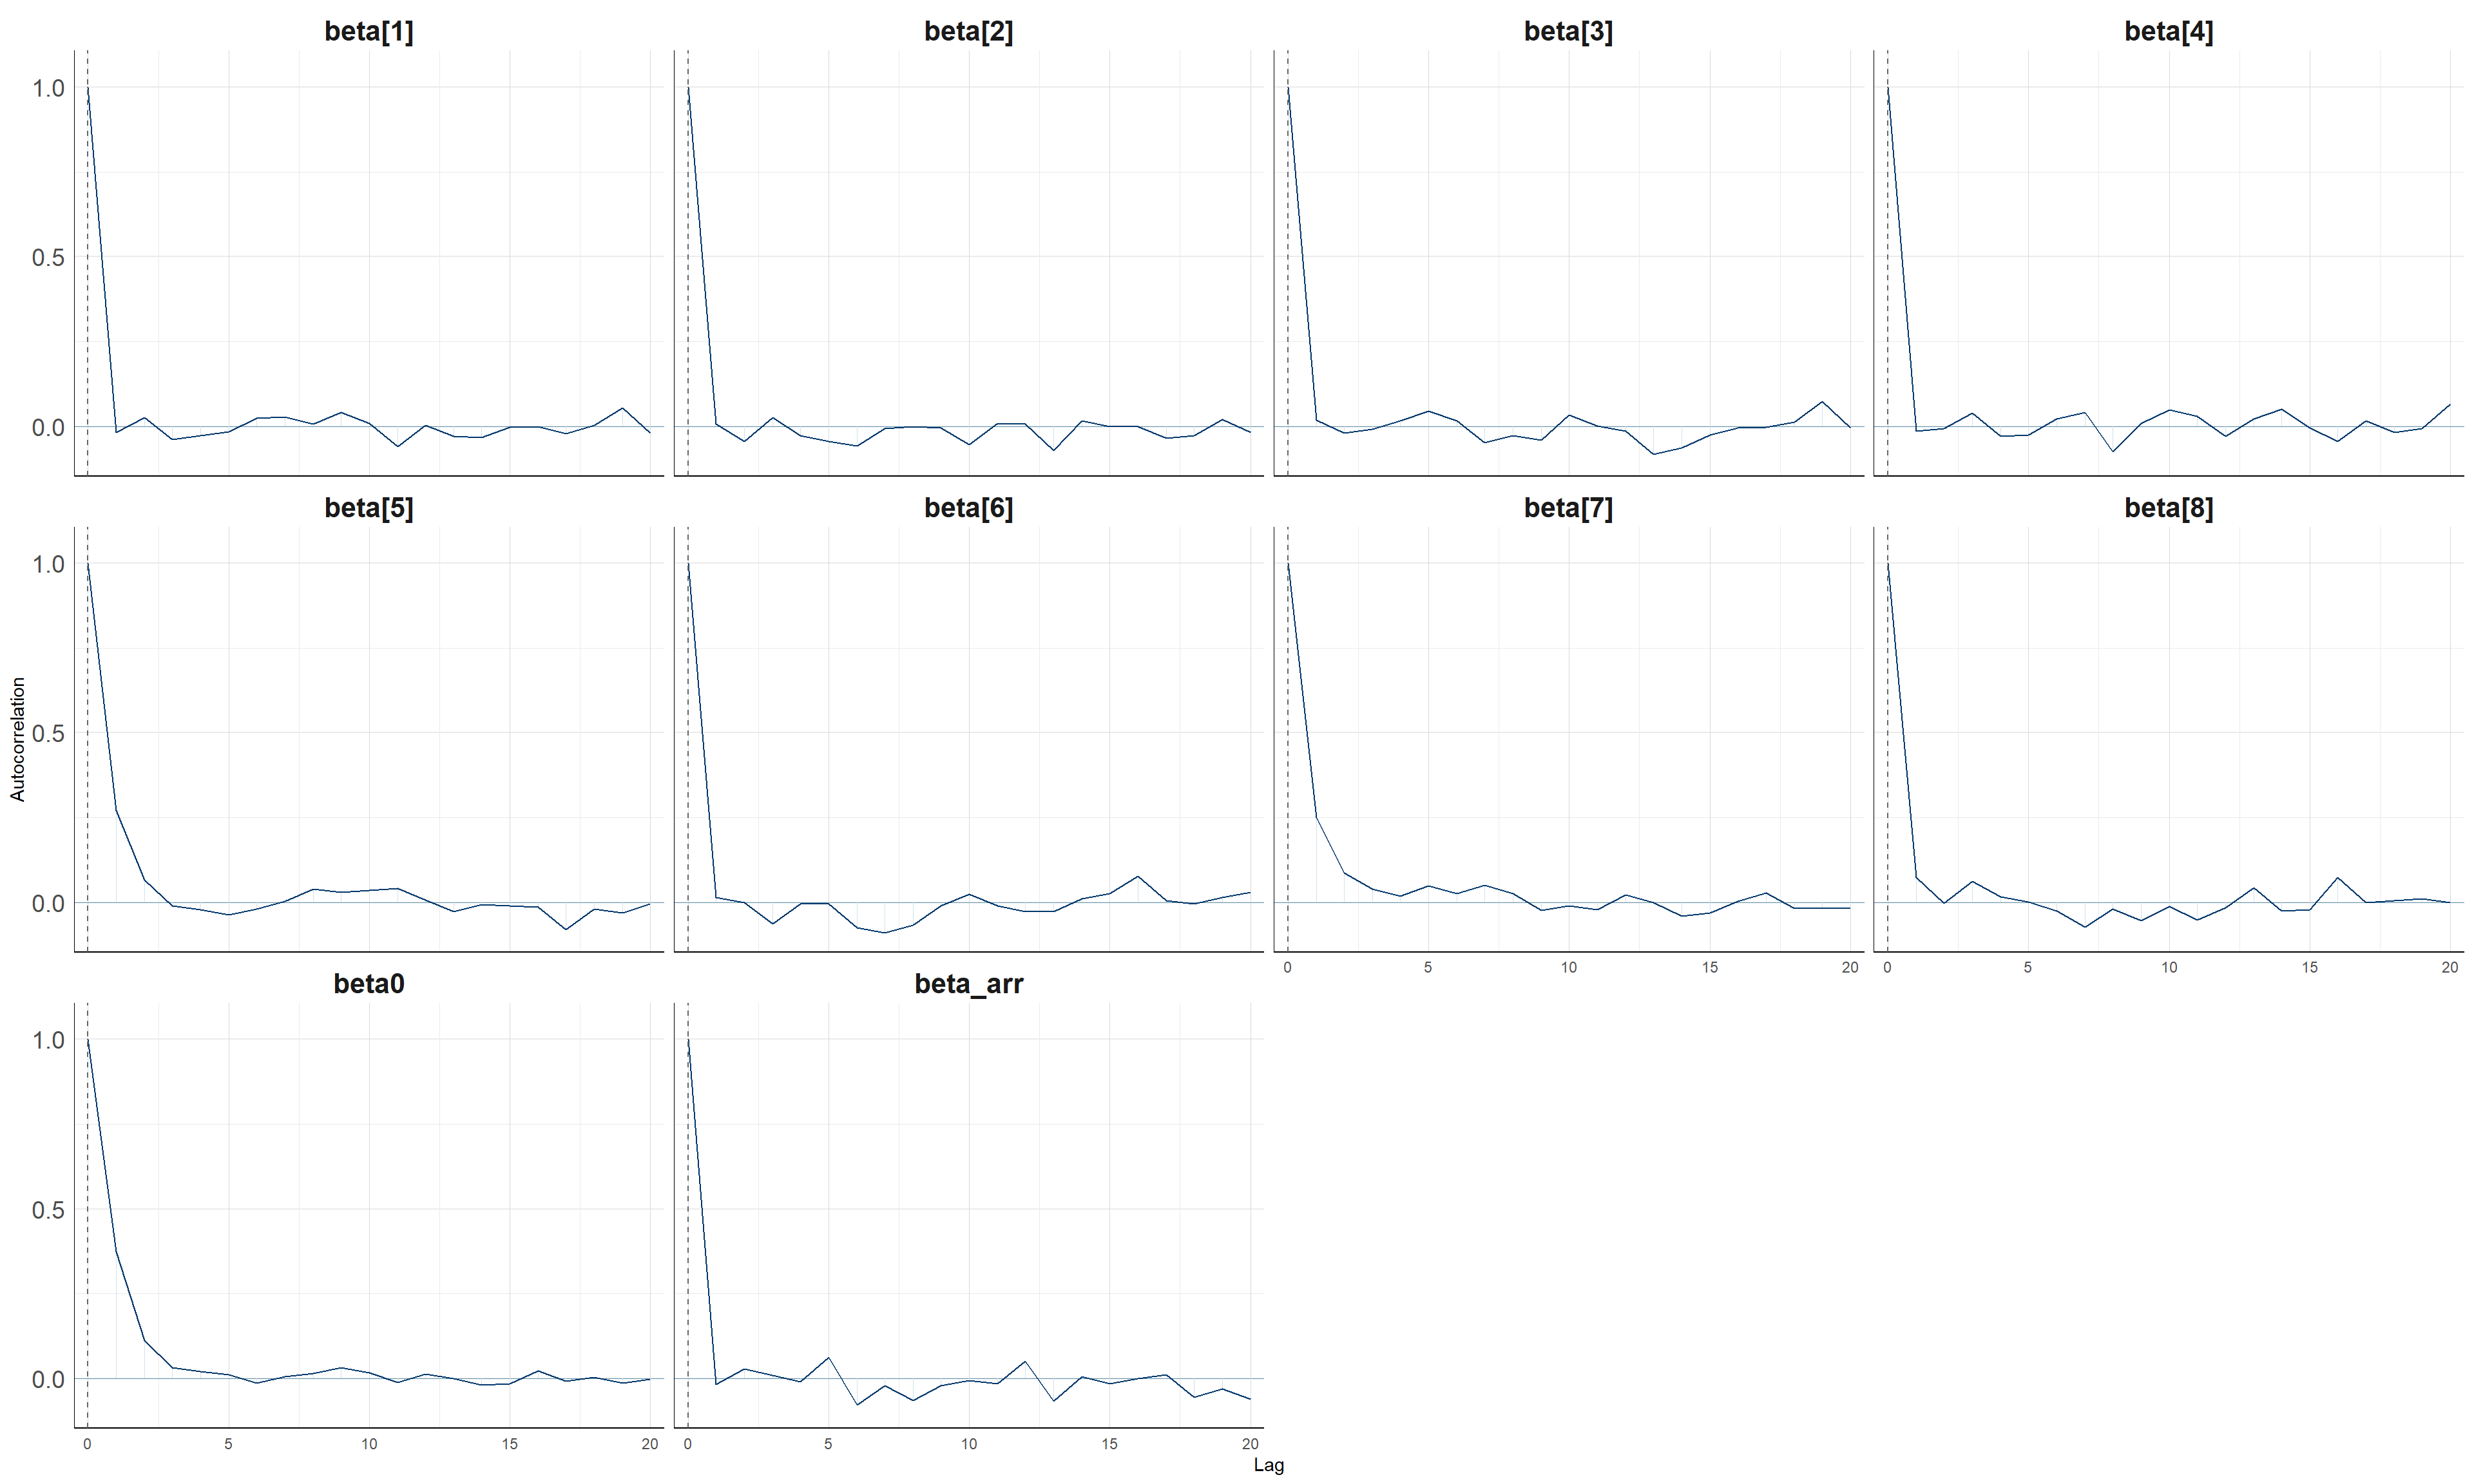
\includegraphics[width=0.7\linewidth]{img/logit_model/acf_1.png}
    \caption{MCMC ACF plots of the baseline logit model (1st chain).}
    \label{fig:logit_acf1}
\end{figure}

\begin{figure}[h]
    \centering
    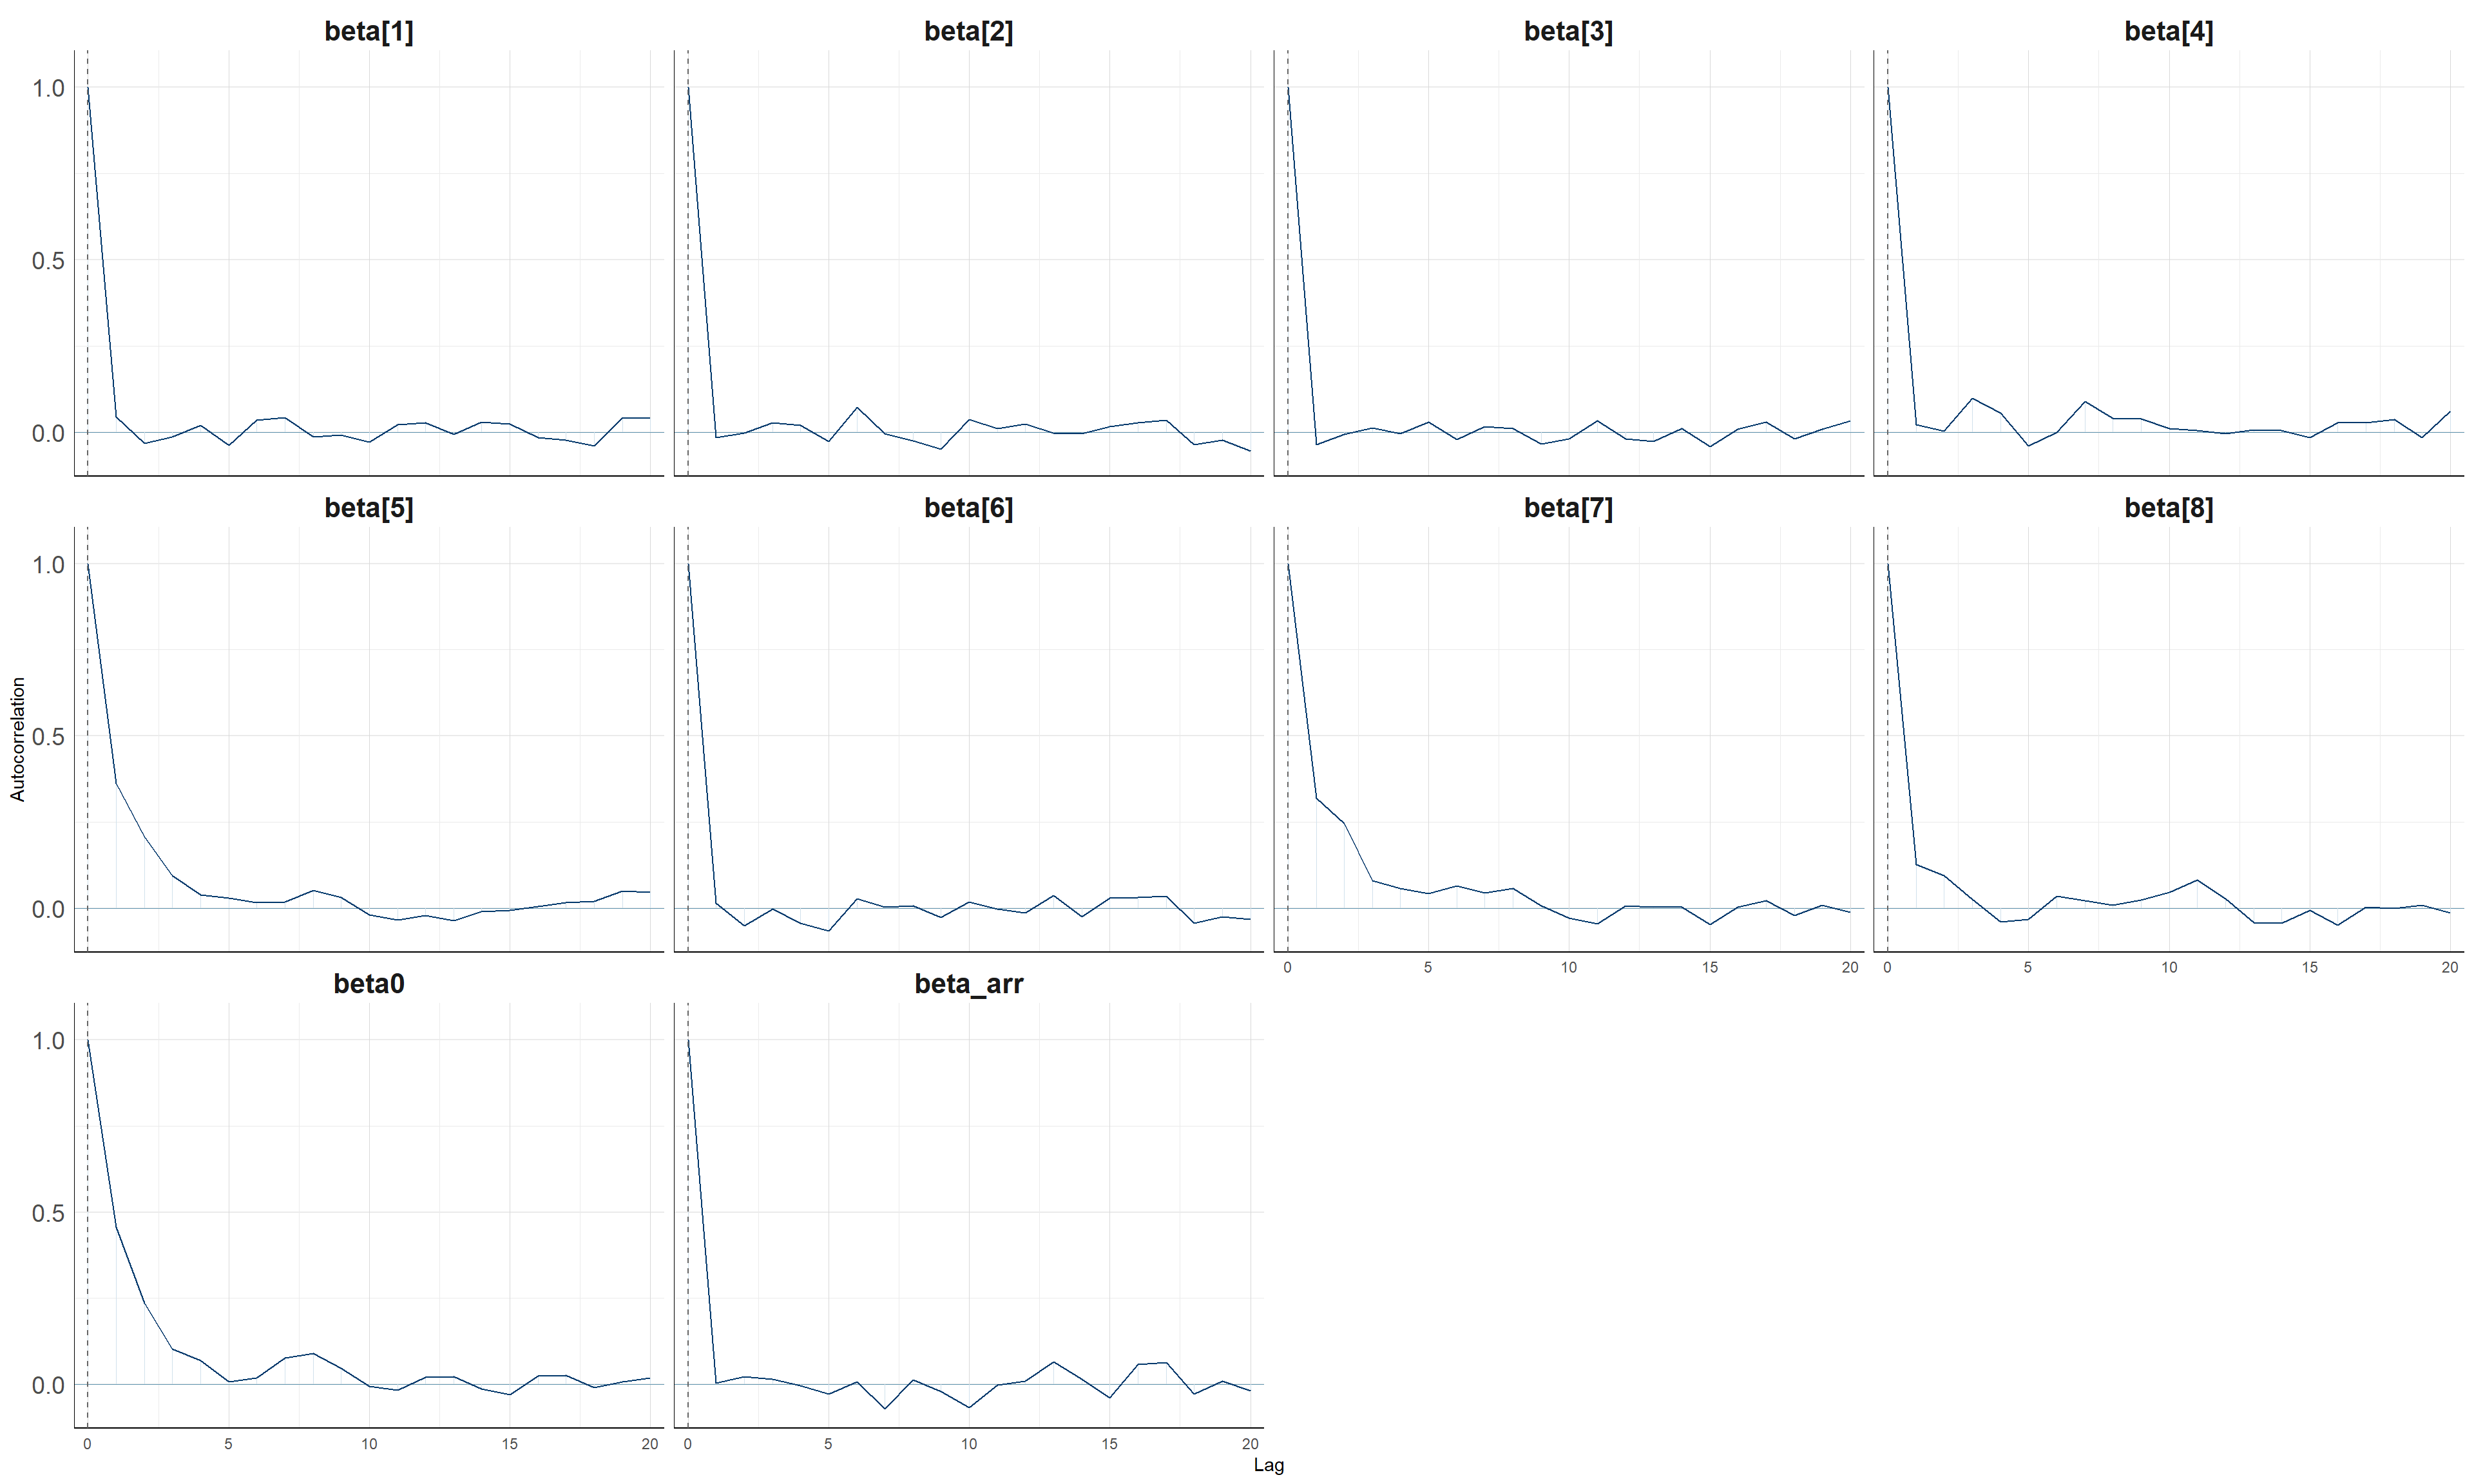
\includegraphics[width=0.7\linewidth]{img/logit_model/acf_2.png}
    \caption{MCMC ACF plots of the baseline logit model (2nd chain).}
    \label{fig:logit_acf2}
\end{figure}

\begin{figure}[h]
    \centering
    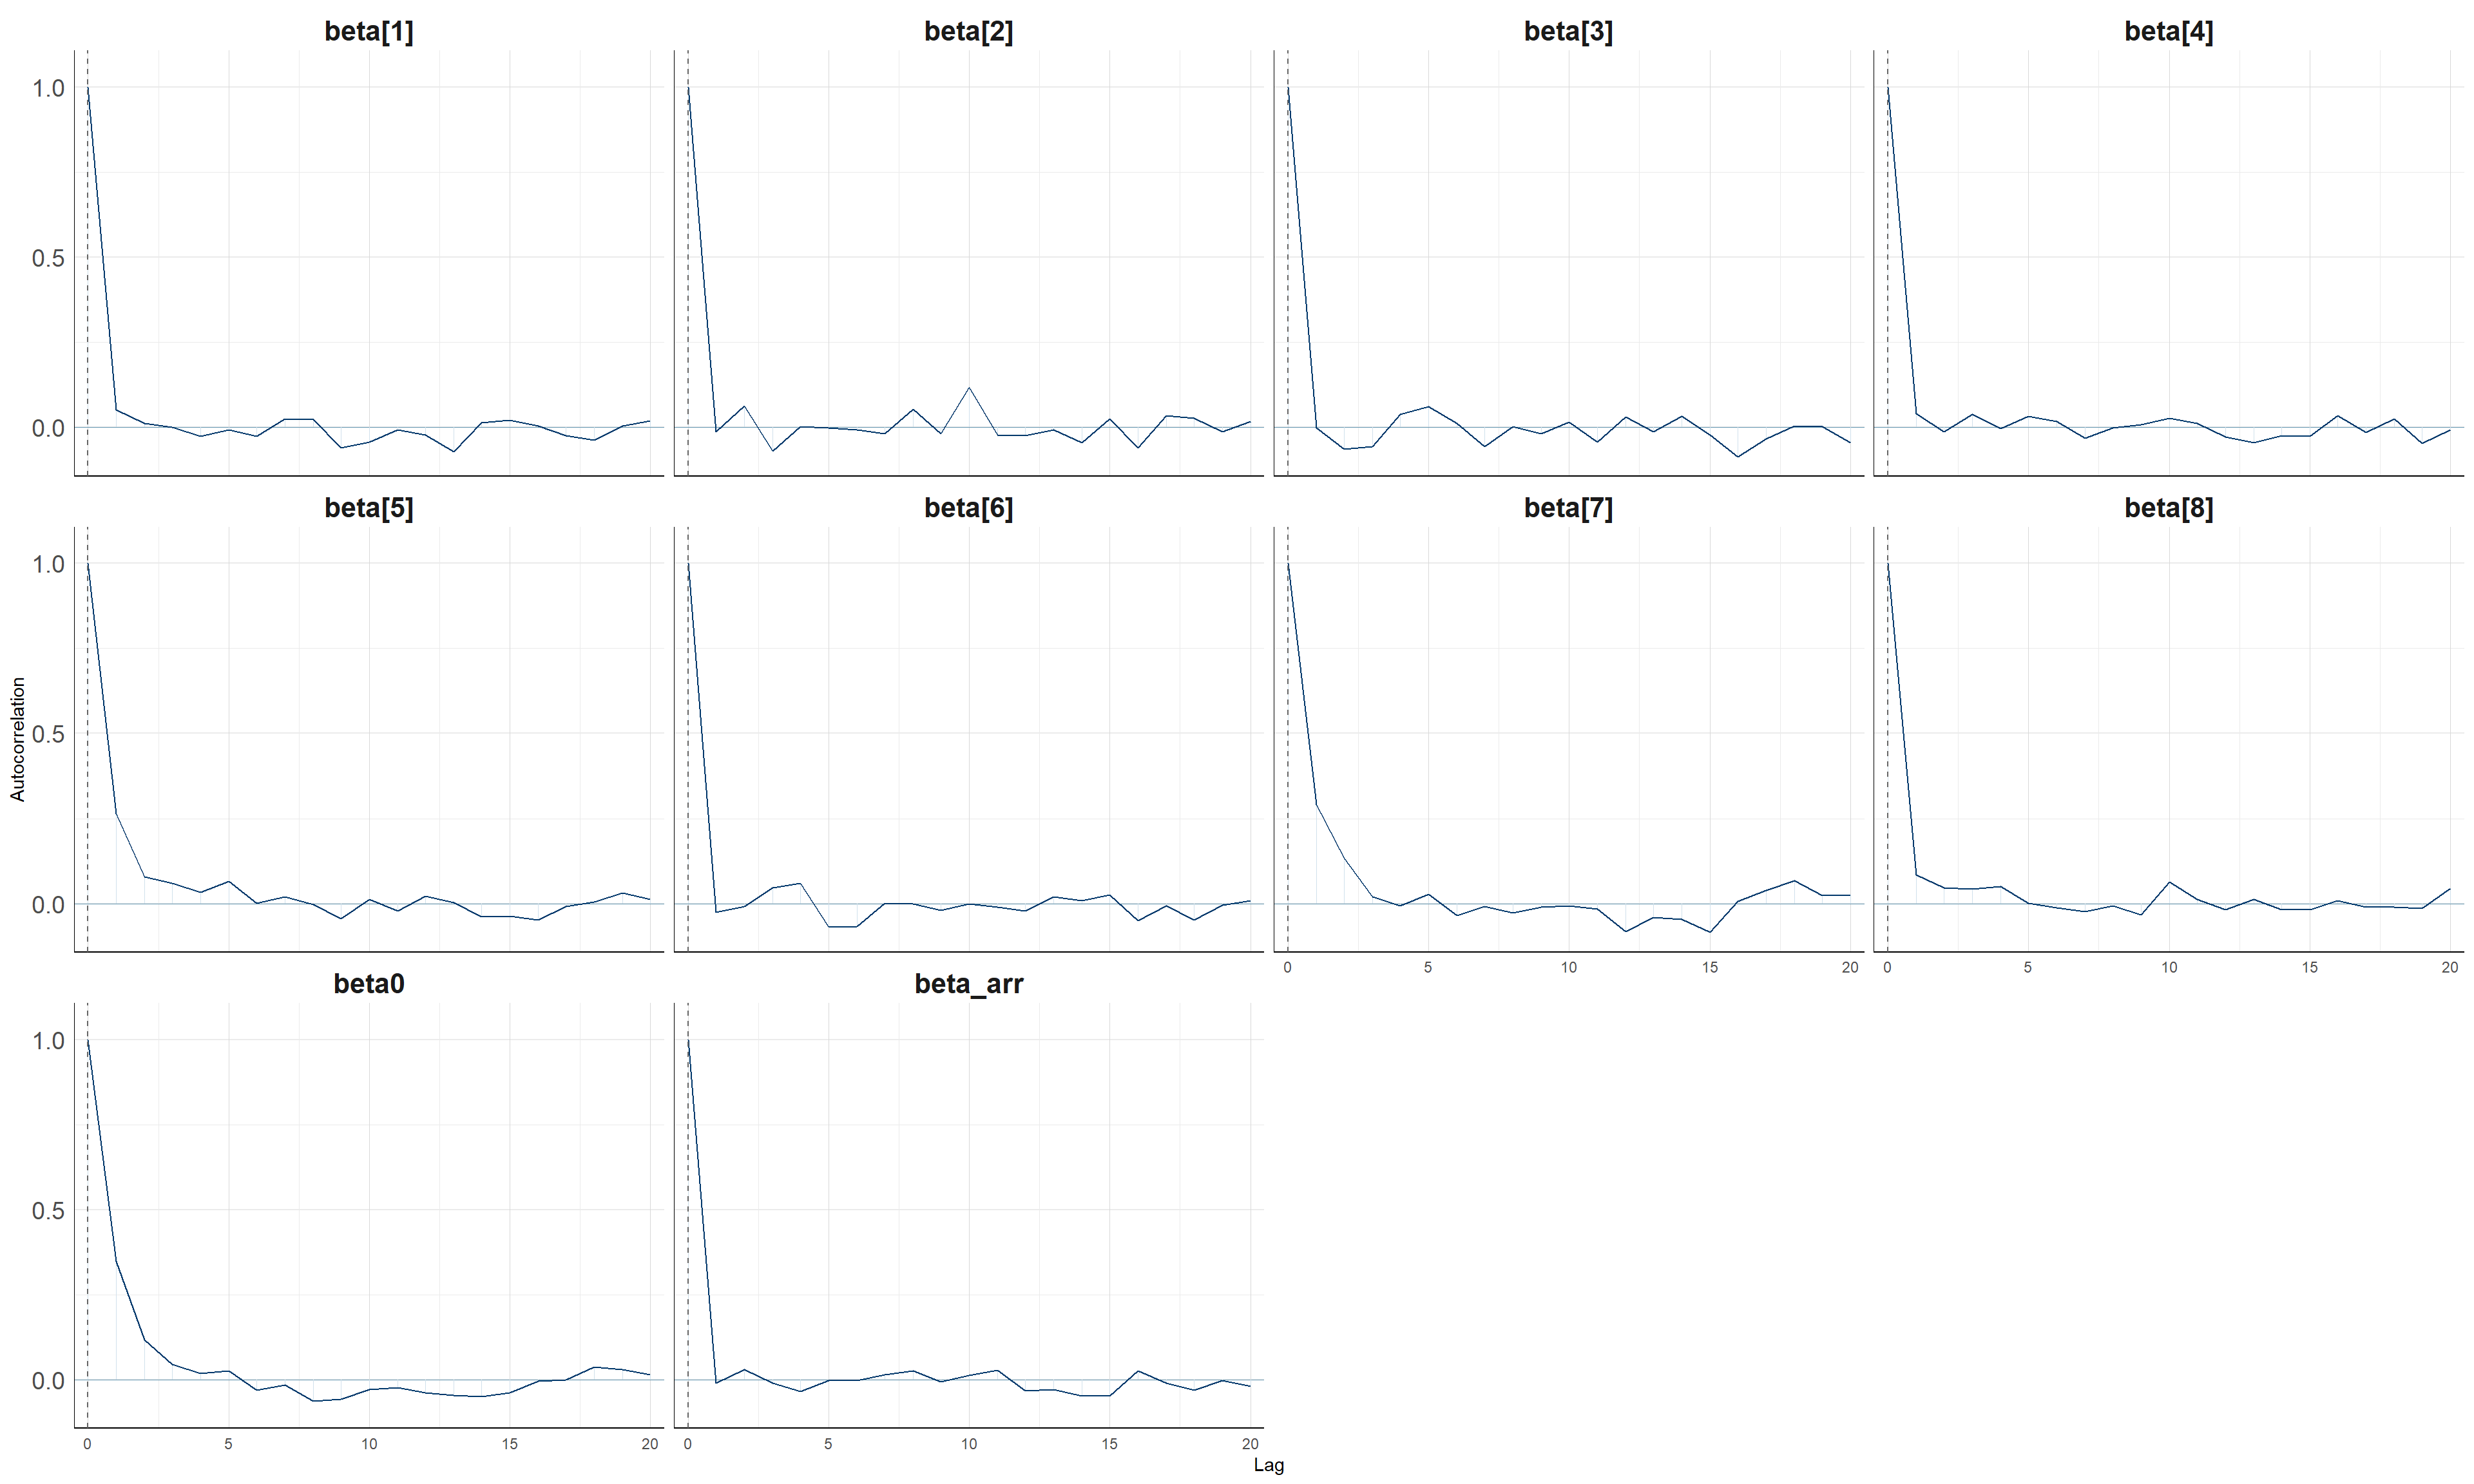
\includegraphics[width=0.7\linewidth]{img/logit_model/acf_3.png}
    \caption{MCMC ACF plots of the baseline logit model (3rd chain).}
    \label{fig:logit_acf3}
\end{figure}

\begin{table}[htbp]
  \centering
  \begin{minipage}[t]{0.48\textwidth}
    \centering
    \captionof{table}{Gelman--Rubin potential scale reduction factors.}
    \label{tab:psrf}
    \begin{tabular}{l S[table-format=1.2] S[table-format=1.2]}
      \toprule
      Parameter & {Point est.} & {Upper C.I.} \\
      \midrule
      $\beta_{1}$      & 1 & 1.00 \\
      $\beta_{2}$      & 1 & 1.00 \\
      $\beta_{3}$      & 1 & 1.00 \\
      $\beta_{4}$      & 1 & 1.01 \\
      $\beta_{5}$      & 1 & 1.00 \\
      $\beta_{6}$      & 1 & 1.01 \\
      $\beta_{7}$      & 1 & 1.00 \\
      $\beta_{8}$      & 1 & 1.01 \\
      $\beta_{0}$      & 1 & 1.01 \\
      $\beta_{\text{arr}}$ & 1 & 1.00 \\
      \midrule
      \multicolumn{3}{l}{\footnotesize Multivariate PSRF: 1} \\
      \bottomrule
    \end{tabular}
  \end{minipage}
  \hfill
  \begin{minipage}[t]{0.48\textwidth}
    \centering
    \captionof{table}{Effective sample sizes.}
    \label{tab:ess}
    \begin{tabular}{l S[table-format=4.3]}
      \toprule
      Parameter & {ESS} \\
      \midrule
      $\beta_{1}$      & 2486.772 \\
      $\beta_{2}$      & 2600.655 \\
      $\beta_{3}$      & 2799.333 \\
      $\beta_{4}$      & 2279.599 \\
      $\beta_{5}$      & 1324.157 \\
      $\beta_{6}$      & 3331.237 \\
      $\beta_{7}$      & 1253.960 \\
      $\beta_{8}$      & 2028.591 \\
      $\beta_{0}$      & 1123.153 \\
      $\beta_{\text{arr}}$ & 2571.000 \\
      \bottomrule
    \end{tabular}
  \end{minipage}
\end{table}
